\setcounter{chapter}{0}

%----------------------------------
\chapter{Introduction}\hyperdef{part}{intro}{}\label{ch:intro}
%----------------------------------


\section{Purpose and Objectives of The \earthlightingDesc}
%%% Incorporate the intro paragraph that used to begin this Chapter here.
%%% This is location of the true introduction where you explain why this
%%% document exists and what it hopes to accomplish.

Simulation is an important tool in the analysis of complex dynamical
systems such as the rendezvous of two spacecraft orbiting the Earth.
Computer animations of these simulations
provide an aid for visualizing and demonstrating the system behaviors.
The imagery portrayed by the computer animated graphics are generated by
simulating cameras aimed at the simulated vehicles. Light from various sources
illuminates the vehicles, making the scene visible to the cameras.

A vehicle in low Earth orbit is subject to three light sources: the sun,
sunlight reflected off of the Earth, and sunlight reflected off of the moon.
The amount of light impinging on a spacecraft from these light sources
varies over time, due to the following factors:

\begin{itemize}
\item The intensity of the sunlight reflected by the Earth or moon
varies with the phase of the Earth or moon.
\item The Earth may obscure either of the two more distant light sources
from view.
\end{itemize}
The purpose of the \earthlightingDesc\ is to model phase variations and
obscuration effects for these three bodies,
thereby providing a measure of realism for the
graphical simulations. The \earthlightingDesc\ accomplishes this by interacting
with a JEOD Dynamics Manager object \cite{dynenv:DYNMANAGER} ,
leveraging information
from the manager to track the current relative
positions of the sun, Earth and moon. A chart of the information flow for
the \earthlightingDesc\ is shown in Figure \ref{flowchart}.

\begin{figure}[H]
\begin{center}
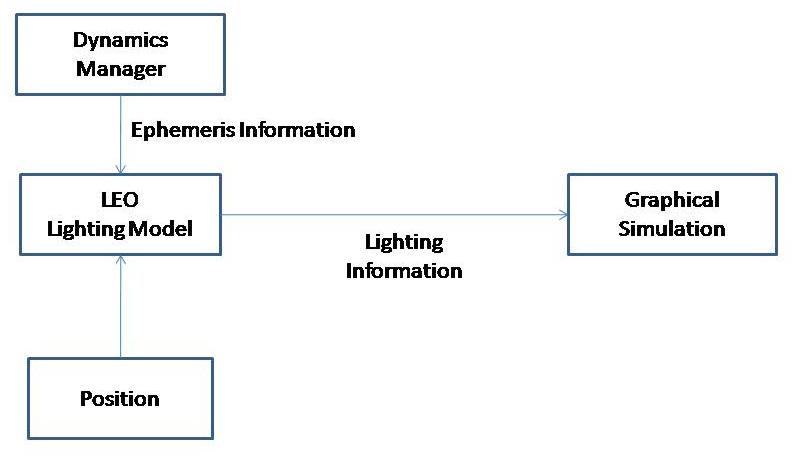
\includegraphics[height=80mm]{pics/flowchart.jpg}
\caption{A Flowchart of Data for the \earthlightingDesc}
\label{flowchart}
\end{center}
\end{figure}

\section{Document History}
%%% Status of this and only this document.  Any date should be relevant to when
%%% this document was last updated and mention the reason (release, bug fix, etc.)
%%% Mention previous history aka JEOD 1.4-5 heritage in this section.

\begin{tabular}{||l|l|l|l|} \hline
\DocumentChangeHistory
\end{tabular}
\\ \\ \\ %%% forced extra space because Latex was formatting oddly.
This document derives heavily from it's predecessor,
JSC Engineering Orbital Dynamics Low Earth Orbit Lighting Model, released with
JEOD v1.5.2.

The following document is parent to this document:
\begin{itemize}
\item{\href{file:\JEODHOME/docs/JEOD.pdf}
           {\em JSC Engineering Orbital Dynamics}}
\cite{dynenv:JEOD}
\end{itemize}

\section{Documentation Organization}
This document is formatted in accordance with the
NASA Software Engineering Requirements Standard~\cite{NASA:SWE}
and is organized into the following chapters:

\begin{description}
%% longer chapter descriptions, more information.

\item[Chapter 1: Introduction] -
This introduction contains four sections; objective and purpose, contex within JEOD, status, and organization.
The section titled objective and purpose provides the true introduction to the \earthlightingDesc\ and its reason
for existance.  The next section identifies the context within JEOD of this document and the \earthlightingDesc.
This is achieved with a directory diagram, a brief description of the interconnections with other models, and
references to any supporting documents.  This is followed by the status of the document which includes
author, date, and reason for each revision.  Finally, there is a description of the how the document is organized.

\item[Chapter 2: Product Requirements] -
Describes requirements for the \earthlightingDesc.

\item[Chapter 3: Product Specification] -
Describes the underlying theory, architecture, and design of the \earthlightingDesc\ in detail.  It will be organized in
three sections; Conceptual Design, Mathematical Formulations, and Detailed Design.

\item[Chapter 4: User Guide] -
Describes how to use the \earthlightingDesc\ in a Trick simulation.  It is broken into three sections to represent the JEOD
defined user types; Analysts or users of simulations (Analysis), Integrators or developers of simulations (Integration),
and Model Extenders (Extension).

\item[Chapter 5: Verification and Validation] -
Contains \earthlightingDesc\ verification and validation procedures and results.

\end{description}

%----------------------------------
\chapter{Product Requirements}\hyperdef{part}{reqt}{}\label{ch:reqt}
%----------------------------------

This chapter identifies the requirements for the \earthlightingDesc.

\requirement{Top-level requirement}
\label{reqt:toplevel}
\begin{description}
\item[Requirement:]\ \newline
  This model shall meet the JEOD project requirements specified in
  the \JEODid\
  \hyperref{file:\JEODHOME/docs/JEOD.pdf}{part1}{reqt}{ top-level
  document}.
\item[Rationale:]\ \newline
  This model shall, at a minimum,  meet all external and internal requirements
  applied to the \JEODid\ release.
\item[Verification:]\ \newline
     Inspection
\end{description}

%%% Format for the model Requirements is open.  It should include requirements for this model
%%% only and use requirment tags like the one below.
%\requirement{...}
%\label{reqt:...}
%\begin{description}
%  \item[...]\ \newline
%    The documentation for the model shall include
%
%    \subrequirement{}
%    \label{reqt:...}
%      Software requirements specification.
%
%    ...
%
%  \item[title]\ \newline
%    text
%
%  ...
%
%\end{description}

\section{Data Requirements}\label{sec:data_reqts}
This section identifies requirements on the data represented by the \earthlightingDesc.
These as-built requirements are based on the \earthlightingDesc\ data definition header
files.

\requirement{Vehicle State Encapsulation}
\label{reqt:data_vehicle_encapsulation}
\begin{description}
  \item[Requirement:]\ \newline
    The \earthlightingDesc\ shall encapsulate the
    descriptions of the sun, Earth, and moon as seen by a spacecraft
    and the extent to which these bodies illuminate the spacecraft
    in a single data object.

  \item[Rationale:]\ \newline
    The overarching purpose  of the \earthlightingDesc\
    is to model the lighting provided by the sun, Earth, and moon
    for use by simulation graphics models.
    This requirement constrains the design of the module data.

  \item[Verification:]\ \newline
    Inspection
\end{description}

\section{Functional Requirements}\label{sec:func_reqts}
This section identifies requirements on the functional
capabilities provided by the \earthlightingDesc.
These as-built requirements are based on the \earthlightingDesc\ source files.

\requirement{Summarize Lighting Bodies}
\label{reqt:func_calc_lighting_bodies}
\begin{description}
  \item[Requirement:]\ \newline
    For each lighting body (the sun, Earth, and moon)
    that illuminates a spacecraft in low Earth orbit,
    the \earthlightingDesc\ shall compute:
  \subrequirement{Relative Position}
  \label{reqt:lighting_body_position}
\\  The position of the lighting body relative to
    the spacecraft.
  \subrequirement{Apparent Size}
  \label{reqt:lighting_body_size}
    \\ The angular size of the lighting body
    as seen from the spacecraft.

  \item[Rationale:]\ \newline
    These calculations are needed by the animated graphics models.

  \item[Verification:]\ \newline
    Inspection, Test
\end{description}

\requirement{Calculate Illumination}
\label{reqt:func_calc_illumination}
\begin{description}
  \item[Requirement:]\ \newline
    For each lighting body that illuminates a spacecraft in LEO, the
    \earthlightingDesc\ shall compute:
  \subrequirement{Occlusion}
    The fraction of the hemisphere of each remote lighting body
    (the Sun and Moon) facing a spacecraft in low Earth orbit
    that is occluded by the Earth as observed by the spacecraft.
  \subrequirement{Lighting}
    The amount of illumination
    provided by each lighting body (the Sun, Earth, and Moon)
    illuminating the spacecraft
    as a fraction of the maximum light provided by that body.
  \item[Rationale:]\ \newline
    These calculations are needed by the animated graphics models.

  \item[Verification:]\ \newline
    Inspection, Test
\end{description}

%----------------------------------
\chapter{Product Specification}\hyperdef{part}{spec}{}\label{ch:spec}
%----------------------------------

This chapter defines the conceptual design, the mathematical formulations, and
the detailed design for the \earthlightingDesc.

\section{Conceptual Design}

\subsubsection{Purpose and Scope}
The \earthlightingDesc\ is designed to compute the lighting environment that a
spacecraft in Earth orbit is experiencing.  It takes in ephemeris information
on the system that the spacecraft is operating in (planetary locations, light
intensity, etc.), as well as information about the current state of the spacecraft,
and uses this information to calculate the lighting
environment.

\subsubsection{Goals and Objectives}
The goal of the \earthlightingDesc\ is to compute the lighting effects that the
spacecraft sees.

\section{Mathematical Formulations}

The \earthlightingDesc\ relies on classical geometric formulations in order
to compute the lighting effects on a body.  It assumes that the only bodies
that are effecting the lighting environment are the Earth, sun, and moon.  In
order to determine what effect these bodies have on the lighting environment,
the spacecraft must first determine if it can ``see" the body.  In other words,
is the body being occluded by the Earth.

\subsection{Body Visibility}
For each of the lighting bodies in question (sun, moon and Earth),
the software has to
determine if the body is completely visible, partially occluded, or completely
blocked by the primary body (Earth). An example of these conditions is shown
below in Figure \ref{lighting_pic}.

\begin{figure}[H]
\begin{center}
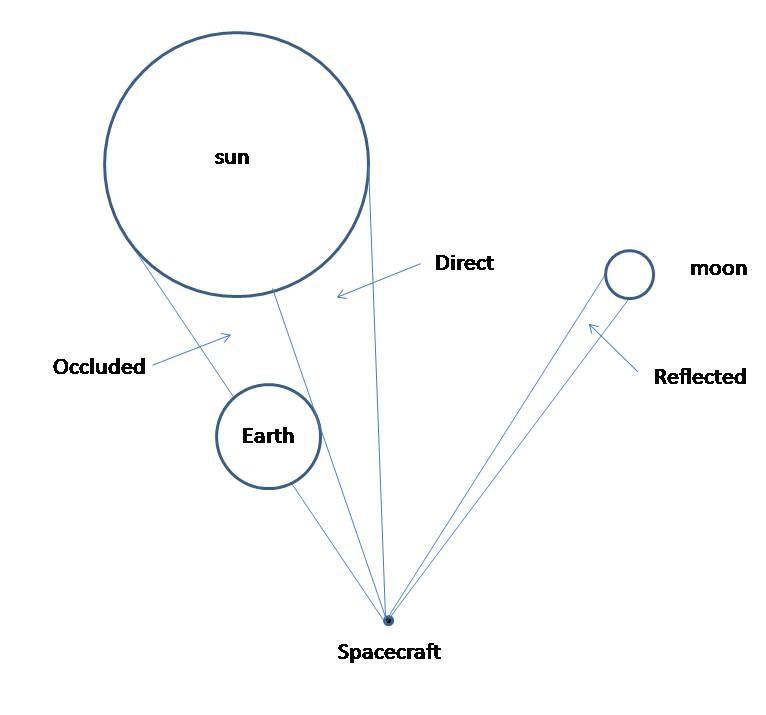
\includegraphics[height=120mm]{pics/lighting_pic.jpg}
\caption{Examples of visible, partially occluded, and reflected light.
Not to scale.}
\label{lighting_pic}
\end{center}
\end{figure}

The software first calculates the angular size of the lighting body disc in the
sky.  In order to do this, it uses the arcsine of the equatorial radius over the
distance from the spacecraft to the lighting body.  This is then stored as the
half-angle for the lighting body.

The software then calculates the body-referenced inertial position vectors from
the spacecraft to the Earth, moon, and sun.  It then uses this information to
calculate the angles between the spacecraft-Earth vector and the spacecraft
sun and moon vectors.

Using all of this information, the software then calculates whether the body
is completely visible, partially occluded, or completely blocked from view.

\subsubsection{Circle Intersection}
The software essentially treats the spacecrafts's field of view like a
unit sphere and
calculates arc-lengths using this unit sphere.  The three arc-lengths of
interest are sent into the circle-intersection function (arc-length of the
Earth-disc half-angle, arc-length of the lighting body half-angle, and arc-
length of the angle between the spacecraft-Earth and spacecraft-lighting body
vectors).  Using these arc-lengths, the software determines what, if any, the
intersections between the lighting body disc and the Earth-disc there are.
The software then sends this information out to the lighting calculation
software.

\subsection{Lighting Effects Calculation}
With the information on the percentage of lighting body occlusion, the software
is then capable of calculating what the lighting effects of that particular
lighting body are.

The software takes the shared area of the two discs and divides this value by
the total area of the lighting body disc to calculate the percentage of the
disc that is occluded by the Earth.  The software then subtracts this from 1
to determine the fraction of the lighting body that is visible.  The final
lighting condition is then a phase fraction multiplied by the visible fraction
to simulate the phases of the moon.


\section{Detailed Design}

The \earthlightingDesc\ uses three classes to accomplish its objectives.
This section will describe these classes in detail.

\subsection{Class Design}

The {\em Earth\_lighting.h} file contains all of the classes
that are used by the \earthlightingDesc\ source code. These classes are
described in the following sections.

\subsubsection{LightingBody}
The class LightingBody contains the information on the
parameters of a lighting body. These parameters are:

\begin{itemize}
\item{radius:} Celestial body mean equitorial radius, in meters,
\item{position:} A three vector of the inertial position of the lighting
body, relative to the observer, in meters,
\item{position:} The distance from the observer to the lighting body, in meters,
\item{half\_angle:} The Apparent half angle of the body disk, in radians.
\end{itemize}

The LightingBody class only contains a default constructor and a destructor,
and has no other member functions.

\subsubsection{LightingParams}
The class LightingParams contains the information on how the lighting body
is affecting the spacecraft. This information is represented by the
following parameters:

\begin{itemize}
\item{obs\_angle:} The apparent observation angle from the light source,
in radians,
\item{phase:} The apparent lighting phase of the planet,
\item{occlusion:} Fraction of planetary surface occlusion,
\item{visible:} Fraction of planetary surface visible,
\item{lighting} Fraction of lighting (phase * visible).
\end{itemize}

The LightingParams class only contains a default constructor and a
destructor, and has no other member functions.

\subsection{EarthLighting}

The EarthLighting class fully defines and calculates the lighting
parameters seen by the vehicle of interest. This class contains the
following parameters:

\begin{itemize}
\item{active:} A booleon flag indicating if the model is active or not,
\item{Earth:} A pointer to a Planet object representing the Earth, obtained
from the DynManager the class is initialized from,
\item{moon:} A pointer to a Planet object representing the moon, obtained
from the DynManager the class is initialized from,
\item{sun:} A pointer to a Planet object representing the sun, obtained
from the DynManager the class is initialized from,
\item{Earth\_frame:} A pointer to the Earth inertial frame, obtained
from the DynManager the class is initialized from,
\item{moon\_frame:} A pointer to the moon inertial frame, obtained
from the DynManager the class is initialized from,
\item{sun\_frame:} A pointer to the sun inertial frame, obtained
from the DynManager the class is initialized from,
\item{sun\_body:} A LightingBody representing the sun stellar parameters.
\item{Earth\_body:} A LightingBody representing the Earth
stellar parameters,
\item{moon\_body:} A LightingBody representing the moon stellar parameters,
\item{sun\_Earth:} A LightingParams representing the lighting of the sun
with respect to the vehicle orbiting the Earth,
\item{moon\_Earth:} A LightingParams representing the lighting of the moon
with respect to the vehicle orbiting the Earth,
\item{Earth\_albedo:} A LightingParams representing the effects of the
Earth albedo on the vehicle.
\end{itemize}

In addition to the default constructor and the destructor,
the EarthLighting class also contains the following member functions.

\paragraph{initialize}

This member function initializes the internal member variables from the
supplied DynManager object.
\begin{itemize}
\item{return:} void - no return
\item{IN:} DynManager\& manager: The DynManager object that contains the
ephemeris for the sun, Earth and moon.
\end{itemize}

\paragraph{circle\_intersect}

This member function calculates the area of an intersection between
two circles, based on the supplied input parameters.
\begin{itemize}
\item{return:} int - Returns 0 for no intersection, 1 for intersection
\item{IN:} double r\_bottom - Radius of the obscured circle.
\item{IN:} double r\_top - Radius of the obscuring circle.
\item{IN:} double d\_centers - Distance between the centers of the circles.
\item{OUT:} double * area - Covered area (the intersection between
the circles).
\end{itemize}

\paragraph{calc\_lighting}

This member function calculates the lighting parameters on the vehicle
at the supplied vehicle position and stores them in the internal
EarthLighting member variables.
\begin{itemize}
\item{return:} void - none
\item{IN:} double pos\_veh[3] - The position of the vehicle of interest,
with respect to the Earth Centered Inertial (ECI) reference frame
\end{itemize}

Further information about the design of this model can be found
in the  \href{file:refman.pdf} {\em Reference Manual}
\cite{earthlightingbib:ReferenceManual}.

\section{Inventory}
All \earthlightingDesc\ files are located in the directory \newline
{\tt \$\{JEOD\_HOME\}/models/environment/earth\_lighting}.
Relative to this directory,
\begin{itemize}
\vspace{-0.2\baselineskip}
\item Header and source files are located
in the model {\tt include} and {\tt src} subdirectories.
Table~\ref{tab:source_files} lists the
configuration-managed files in these directories.
\vspace{-0.1\baselineskip}
\item Documentation files are located in the model {\tt docs} subdirectory.
See table~\ref{tab:documentation_files}
for a listing of the
configuration-managed files in this directory.
\vspace{-0.1\baselineskip}
\item Verification files are located in the model {\tt verif} subdirectory.
See table~\ref{tab:verification_files}
for a listing of the
configuration-managed files in this directory.
\end{itemize}

\input{inventory}

%----------------------------------
\chapter{User Guide}\hyperdef{part}{user}{}\label{ch:user}
%----------------------------------
The Analysis section of the user guide is intended primarily for users of pre-existing simulations.
It contains:
\begin{itemize}
\item A description of how to modify \earthlightingDesc\ variables after the simulation
has compiled, including an in-depth discussion of the input file,
\item An overview of how to interpret (but not edit) the S\_define file,
\item A sample of some of the typical variables that may be logged.
\end{itemize}

The Integration section of the user guide is intended for simulation developers.
It describes the necessary configuration of the \earthlightingDesc\ within an
S\_define file, and the creation of standard run directories.  The Integration
section assumes a thorough understanding of the preceding Analysis section of the user guide.
Where applicable, the user may be directed to selected portions of Product Specification (Chapter \ref{ch:spec}).

The Extension section of the user guide is intended primarily for developers
needing to extend the capability of the \earthlightingDesc.  Such users should have a
thorough understanding of how the model is used in the preceding
Integration section, and of the model
specification (described in Chapter \ref{ch:spec}).

Note that the \earthlightingDesc\ depends heavily on the Dynamics Manager
(DynManager) class, and any simulation involving a \earthlightingDesc\ object
will require the successful setup of a DynManager object \cite{dynenv:DYNMANAGER}.

\section{Analysis}

The Analysis and the Integration sections will assume, for the purposes of
illustration, an S\_define object of the following form:

\begin{verbatim}
 sim_object {

   environment/Earth_lighting: EarthLighting lighting;

   double position[3]; /*spacecraft position*/


   P_ENV (initialization) environment/Earth_lighting:
      LIGHT.lighting.initialize(
      In DynManager& manager = mngr.dyn_manager);


   /* Call the lighting source code */
   (DYNAMICS, scheduled) environment/Earth_lighting:
      LIGHT.lighting.calc_lighting(
      In    double    pos_veh[3]   = &LIGHT.position[0]);

} LIGHT;
\end{verbatim}

The S\_define will also contain an accompanying sim object titled 'mngr'
containing an appropriately named DynManager instantiation.

The input files for the \earthlightingDesc\ are straight-forward.
The only information not directly pulled from the supplied DynManager object
is the current phase of the moon and the sun, as seen from
the Earth. In the above example code, these
parameters can be set with the input file commands:

\begin{verbatim}
LIGHT.lighting.sun_Earth.phase = 1;
LIGHT.lighting.moon_Earth.phase = 1;
\end{verbatim}

Note that the phase stated here simulates the fraction of the lighting body
that is actually radiating light. In the moon's case this value can range
from 0-1. In the case of the sun, this value should always be 1.


\section{Integration}

Integrating the \earthlightingDesc\ into an S\_define is a simple process.
An EarthLighting object must first be instantiated, as shown in the first
lines of the example code in the Analysis section above.

Before the \earthlightingDesc\ can be used to calculate lighting
characteristics, it must be initialized using a correctly instantiated
and initialized DynManager object. The following code gives an example
of this initialization:

\begin{verbatim}
P_ENV (initialization) environment/Earth_lighting:
   LIGHT.lighting.initialize(
   In DynManager& manager = mngr.dyn_manager);
\end{verbatim}

Note that the DynManager object must be initialized before this function is called.
Also, the \earthlightingDesc\ requires that the DynManager object used
for initialization contains three Planet objects, with the following
specific names: ``Earth", ``Moon", and ``Sun". If
this requirement is not met, then the \earthlightingDesc\ initialization
function will fail and produce an error message. Information on correctly
initializing can be found in the DynManager documentation \cite{dynenv:DYNMANAGER}.

Finally, the specific lighting information can be calculated with the
following call.

\begin{verbatim}
(DYNAMICS, scheduled) environment/Earth_lighting:
   LIGHT.lighting.calc_lighting(
   In    double    pos_veh[3]   = &LIGHT.position[0]);
\end{verbatim}

The input is the current position of the vehicle in the ECI
 frame. For most simulations where the use of the
\earthlightingDesc\ is appropriate, this will be the default integration
frame, and the position can be obtained from the appropriate DynBody object
\cite{dynenv:DYNBODY}. However, if the integration
frame is not the ECI frame, the correct position of the vehicle can be
obtained using the JEOD reference frame utilities combined
with the DynManager \cite{dynenv:DYNMANAGER} object.
This position can also be determined using
a user define DerivedState object \cite{dynenv:DERIVEDSTATE}.

\section{Extension}

The current implemention of the \earthlightingDesc\ depends heavily on the
assumption of low Earth orbit, and is not intended to be extendable to other
space environments.


%----------------------------------
\chapter{Verification and Validation}\hyperdef{part}{ivv}{}\label{ch:ivv}
%----------------------------------

\section{Verification}
%%% code imported from old template structure
%\inspection{<Name of Inspection>}\label{inspect:<label>}
% <description> to satisfy
% requirement \ref{reqt:<label>}.

\inspection{Top-level inspection}\label{inspect:TLI}
 This document structure, the code, and associated files have been inspected, and together satisfy requirement \ref{reqt:toplevel}.


\inspection{Data conversion}\label{inspect:data_conversion}
By inspection, the data structures of the \earthlightingDesc\ completely satisfy
requirement \ref{reqt:data_vehicle_encapsulation}.


\section{Validation}
In each test case, simulations were run with different input files.  Each
individual input file has its own associated run directory.  These run
directories are named with the convention RUN\_T\#\#\_LIGHT\_VER where the
\#\# characters are replaced by a 2-digit number.  These run directories are
contained in the SET\_test sub-directory of SIM\_LIGHT\_CIR.

\test{Identical Circle Intersection}\label{test:ident_cir}
\begin{description}
\item[Purpose:] \ \newline
This test case is designed to examine the performance of the circle
intersection calculation with two circles that have the same radius
and are located adjacent to each other.
\newline
Run directory: RUN\_T01\_LIGHT\_VER (Test 1)\newline
               RUN\_T02\_LIGHT\_VER (Test 2)\newline
               RUN\_T03\_LIGHT\_VER (Test 3)\newline
               RUN\_T04\_LIGHT\_VER (Test 4)\newline
               RUN\_T05\_LIGHT\_VER (Test 5)\newline
\item[Requirements:]% \ \newline
By passing this test, this model partially satisfies requirements
\mbox{\ref{reqt:func_calc_lighting_bodies}}, and
\mbox{\ref{reqt:func_calc_illumination}}.

\item[Procedure:]\ \newline
To test the capabilities of the circle\_intersect function included in
the lighting model, a MATLAB script was written that will test the area
calculation function by completely separate means.  The x and y coordinates
for two circles were generated using an array of angles and the sin and cos
functions.  The points of intersection for these two circles were then
calculated analytically.  Using this intersection information, a polygon was
generated from the points forming the common area.  The area of this polygon
was calculated, using MATLAB's polyarea function and compared with the
analytical output from the function.  A plot of the circle intersection for
the first set of parameters from Table \ref{equi_rad_table} can be seen in
Figure \ref{cool_circle_plot}.

\begin{figure}[H]
\begin{center}
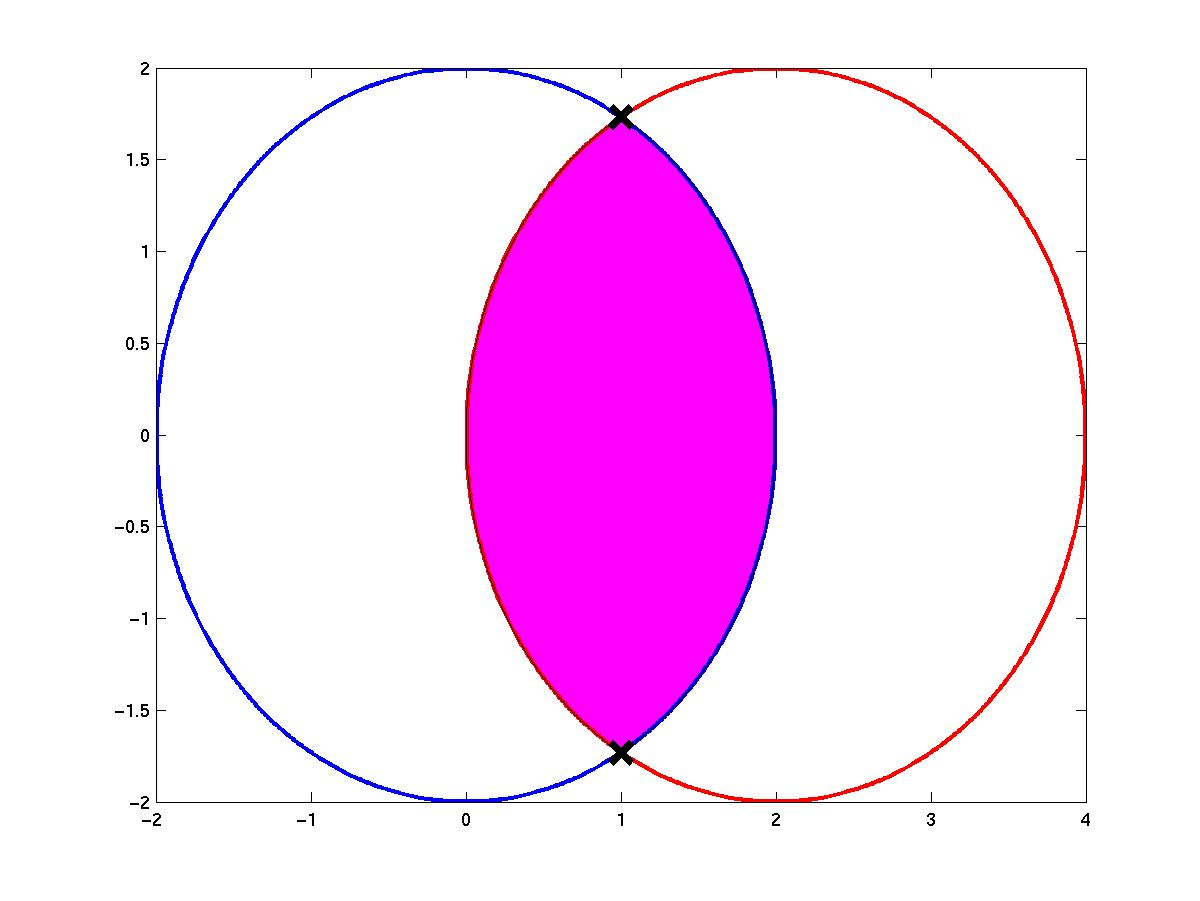
\includegraphics[height=80mm]{pics/circle_area1.jpg}
\caption{Circle Intersection Illustration}
\label{cool_circle_plot}
\end{center}
\end{figure}

\item[Results:]\ \newline
Table \ref{equi_rad_table} shows the results of the various tests run for
various circle parameters.
\begin{table}[ht]
\begin{tabular}{|l|l|l|l|l|l|l|}\hline
 Test & $r_{top}$ ($m$) & $r_{bot}$ ($m$) & $d_{cent}$ ($m$) & Model Output ($m^2$) &
    MATLAB ($m^2$) & Difference ($m^2$) \\ \hline
 1 & 2.0 & 2.0 & 2.0 & 4.913 & 4.913 & 1.68E-7 \\ \hline
 2 & 3.0 & 3.0 & 1.0 & 22.302 & 22.302 & 4.77E-7 \\ \hline
 3 & 1.5 & 1.5 & 1.25 & 0.563 & 0.563 & 6.96E-8 \\ \hline
 4 & 0.25 & 0.25 & 1.0 & 0 & 0 & 0 \\\hline
 5 & 4.0 & 4.0 & 0.0 & 50.266 & 50.266 & 0 \\ \hline
\end{tabular}
\caption{Table of Circle Intersection Parameters for First Test}
\label{equi_rad_table}
\end{table}

As this table shows, the model performed correctly in every case.  The level
of error seen in each sub-test is due to the discretization of the circles used
in the MATLAB function.  In the final two tests, the MATLAB function was not
able to calculate the common area because there were no intersections between
the circles.  However, since in test 4 there was no common area, and in test
5, the circles were directly on top of each other, the correct value was easy
to determine.
\end{description}

% asdf   \\ %%% forced space because Latex was placing weird
\test{Different Circle Intersection}\label{test:diff_cir}
\begin{description}
\item[Purpose:] \ \newline
This test case is designed to examine the performance of the circle
intersection calculation with two circles that have the same radius and
are located adjacent to each other.
\newline
Run directory: RUN\_T06\_LIGHT\_VER (Test 6) \newline
               RUN\_T07\_LIGHT\_VER (Test 7) \newline
               RUN\_T08\_LIGHT\_VER (Test 8) \newline
               RUN\_T09\_LIGHT\_VER (Test 9) \newline
               RUN\_T10\_LIGHT\_VER (Test 10) \newline
\item[Requirements:]% \ \newline
By passing this test, this model partially satisfies requirements
\mbox{\ref{reqt:func_calc_lighting_bodies}}, and
\mbox{\ref{reqt:func_calc_illumination}}.

\item[Procedure:]\ \newline
To test, the capabilities of the circle\_intersect function included in the
lighting model, a MATLAB script was written that tested the area
calculation function by completely separate means.  The x and y coordinates
for two circles were generated using an array of angles and the sin and cos
functions.  The points of intersection for these two circles were then
calculated analytically.  Using this intersection information, a polygon was
generated from the points forming the common area.  The area of this polygon
was calculated using MATLAB's polyarea function and compared with the
analytical output from the function.  A plot of the circle intersection for
the first set of parameters from Table \ref{diff_rad_table} can be seen in
Figure \ref{diff_circle_plot}.

\begin{figure}[H]
\begin{center}
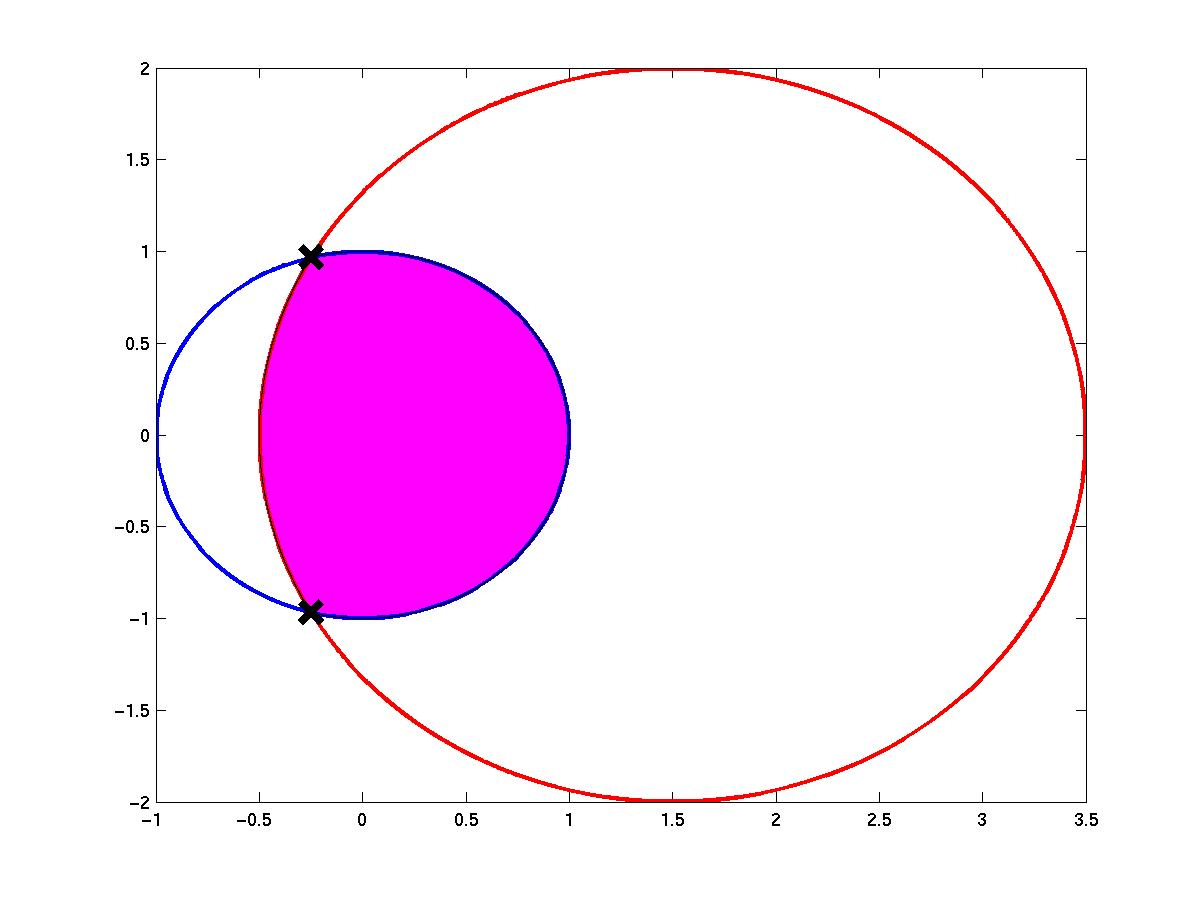
\includegraphics[height=80mm]{pics/circle_area2.jpg}
\caption{Circle Intersection Illustration for Different Radius}
\label{diff_circle_plot}
\end{center}
\end{figure}

\item[Results:]\ \newline
Table \ref{diff_rad_table} shows the results of the various tests run for
various circle parameters.
\begin{table}[ht]
\begin{tabular}{|l|l|l|l|l|l|l|}\hline
Test & $r_{top}$ ($m$) & $r_{bot}$ ($m$) & $d_{cent}$ ($m$) & Output ($m^2$) &
   MATLAB ($m^2$) & Difference ($m^2$) \\ \hline
6 & 1.0 & 2.0 & 1.5 & 2.393 & 2.393 & 8.96E-8 \\ \hline
7 & 3.0 & 1.5 & 2.0 & 6.084 & 6.084 & 2.76E-7 \\ \hline
8 & 3.0 & 1.5 & 4.25 & 0.233 & 0.233 & 1.69E-7 \\ \hline
9 & 3.0 & 1.5 & 1.75 & 6.693 & 6.693 & 1.93E-7 \\ \hline
10 & 3.0 & 2.0 & 0.5 & 12.566 & 12.566 & 2.07E-7 \\ \hline
\end{tabular}
\caption{Table of Circle Intersection Parameters for Second Test}
\label{diff_rad_table}
\end{table}

As this table shows, the model once again performed correctly even with circles
of different radius as inputs.  Note that in the final test, the bottom circle
was completely occluded by the top circle.  In this case, the MATLAB function
did calculate the area correctly and so the discretization error is seen here
again.

\end{description}

\test{Planetary Disc Intersection}\label{test:plan_disc}
\begin{description}
\item[Purpose:] \ \newline
This test case is designed to examine the performance of the lighting
function when the sun is partially occluded by the Earth.
\newline
Run directory: RUN\_T01\_LIGHT\_VER \newline
\item[Requirements:] % \ \newline
By passing this test, this model partially satisfies requirements
\mbox{\ref{reqt:func_calc_lighting_bodies}}, and
\mbox{\ref{reqt:func_calc_illumination}}.

\item[Procedure:]\ \newline
This test is designed to ensure that the code correctly computes the fraction
of the sun's area that is visible when the sun is partially occluded by the
Earth.  All planetary radii were set to 1 m, the spacecraft was
placed at (-2, 0, 0) m, the sun at (1, .75, 0) m, the moon at (1, -.75, 0) m,
and all planetary phases were set to 0.
\item[Results:]\ \newline
The major outputs of the lighting model will be detailed here.  It is expected
that from this test, the half-angles of both the sun and the moon will be
calculated as 18.87 degrees.  The model computed these angles correctly out to
machine precision.

The half-angle of the Earth in this case should be 30 degrees and this was
also computed correctly out to machine precision.

The observation angle between the Earth-vector and the sun-vector should then
be 14.036 degrees.  This value was also calculated to machine precision.  The
moon observation vector should also equal this value, and this was calculated
correctly as well.

With this data, the function should correctly calculate the occluded area for
each of the planetary bodies.  In this case, the values will be the same for
both the sun and the moon, and should be equal to .3226.
This value is not recorded in the
simulation, but it was checked with a debugger and agreed with the values
out to the expected precision.

The fraction of the occluded area should then be this value divided by the
total area of the body on the unit sphere which is equal to .947 and the
visible area should be equal to 1 minus this value.  In both cases, the
results output from the simulation were accurate to the expected precision.
The final lighting fraction should be zero based on the phase value of zero
used in simulation and this was correct as well.

\end{description}

\test{Complete moon Occlusion}\label{test:moon_occlud}
\begin{description}
\item[Purpose:] \ \newline
This test case is designed to examine the performance of the lighting
function when the sun is partially occluded by the Earth.
\newline
Run directory: RUN\_T02\_LIGHT\_VER \newline
\item[Requirements:]% \ \newline
By passing this test, this model partially satisfies requirements
\mbox{\ref{reqt:func_calc_lighting_bodies}}, and
\mbox{\ref{reqt:func_calc_illumination}}.

\item[Procedure:]\ \newline
This test is designed to ensure that the code correctly computes the fraction
of the sun's area that is visible when the sun is partially occluded by the
Earth.  All planetary radii were set to 1 m, the spacecraft was
placed at (-2, 0, 0) m, the sun at (1, 1.5, 0) m, the moon at (1, 0, 0) m, and
all planetary phases were set to 1.
\item[Results:]\ \newline
In this test, the moon should be completely occluded.  The sun should have a
new observation angle calculated as 26.57 degrees.  This value was calculated
out to machine precision by the model.

The moon should be completely occluded by the Earth and it was according to
the code.

The sun should be partially occluded albeit with a different value due to its
new position in the sky.  The sun was in a different position and the
calculated occluded fraction should be equal to .56137, and it agreed with the
MATLAB calculation out to the expected 8 digits of precision.

Once again, the model preformed exactly as expected.

\end{description}

\test{Full Sun Exposure}\label{test:sun_behind}
\begin{description}
\item[Purpose:] \ \newline
This test case is designed to examine the performance of the lighting
function when the sun is not occluded by the Earth.
\newline
Run directory: RUN\_T03\_LIGHT\_VER \newline
\item[Requirements:]% \ \newline
By passing this test, this model partially satisfies requirements
\mbox{\ref{reqt:func_calc_lighting_bodies}}, and
\mbox{\ref{reqt:func_calc_illumination}}.

\item[Procedure:]\ \newline
This test is designed to ensure that the code correctly computes the fraction
of the sun's area that is visible when the sun is not occluded.
All planetary radii were set to 1 m except for the moon's which was
set to 2 m, the spacecraft was placed at (-2, 0, 0) m, the sun at (-3, 0.0, 0)
m, the moon at (1, 1.5, 0) m, and all planetary phases were set to 0.5.
\item[Results:]\ \newline
In this test, the sun should be completely visible to the spacecraft.  The
moon should be partially occluded by the Earth although it will have a larger
visible area than in the first test because of its increased radius.  The
Earth-Albedo effect in this case should be equal to the value of the Solar
fraction.

The new lunar half-angle should be equal to 36.604 degrees, and this value
matched the expected value to machine precision.  The larger visible area
should be equal to .5294, and this agreed out to the expected precision.
The occluded and visible fraction agreed with the correct values (0.4128
and 0.5871) out to the expected precision.  And the lighting fraction was
then half of this value, as expected.

The Earth-Albedo effects were then calculated to the best of the code's
abilities.  The calculated fraction was 0.5.  It is important to note this
behavior here.  When calculating the Earth-Albedo effects, the code basically
takes the fraction of the Solar radiation normal to the surface of the Earth
and uses this value for the Earth-Albedo fraction.  There is no correction
factor applied, so the Earth is essentially treated as a perfect reflector.
This is a bad approximation and will make results inaccurate if used blindly.
However, for the intended purposes of this model, to give approximate lighting
effects only for visualization and not for analytical engineering, this
approximation can be used successfully. Otherwise the user must be aware of the
method's limitations, and not use this approximation for any application where
precision engineering is required.


\end{description}

\section{Metrics}
\subsection{Code Metrics}

Table~\ref{tab:coarse_metrics} presents coarse metrics on the
source files that comprise the model.

\input{coarse_metrics}

Table~\ref{tab:metrix_metrics} presents the extended cyclomatic
complexity
(ECC) of the methods defined in the model.
\input{metrix_metrics}


\section{Requirements Traceability}\label{sec:traceability}

\begin{longtable}[c]{||p{3in}|p{3in}|}
\caption{Requirements Traceability} \\[6pt]
\hline
{\bf Requirement} & {\bf Inspection and Testing} \\
\hline \hline
\endfirsthead
\hline
\endfoot
\caption[]{Requirements Traceability (continued)} \\[6pt]
\hline
{\bf Requirement} & {\bf Inspection and Testing} \\
\hline \hline
\endhead

\ref{reqt:toplevel} - Top-level Requirements &
  Insp.~\ref{inspect:TLI} \\
  \hline

\ref{reqt:data_vehicle_encapsulation} - Vehicle State Encapsulation &
   Insp.~\ref{inspect:data_conversion} \\
\hline

\ref{reqt:func_calc_lighting_bodies} - Summarize Lighting Bodies &
   Test~\ref{test:ident_cir} \\
   &Test~\ref{test:diff_cir} \\
   &Test~\ref{test:plan_disc} \\
   &Test~\ref{test:moon_occlud} \\
   &Test~\ref{test:sun_behind} \\
\hline

\ref{reqt:func_calc_illumination} - Calculate Illumination &
   Test~\ref{test:ident_cir} \\
   &Test~\ref{test:diff_cir} \\
   &Test~\ref{test:plan_disc} \\
   &Test~\ref{test:moon_occlud} \\
   &Test~\ref{test:sun_behind} \\
\hline

\end{longtable}
